\documentclass[12pt,a4paper]{article}
\usepackage[utf8]{inputenc}
\usepackage[greek,english]{babel}
\usepackage{alphabeta} 
\usepackage[pdftex]{graphicx}
\usepackage[top=1in, bottom=1in, left=0.5in, right=0.5in]{geometry}
\linespread{1}
\setlength{\parskip}{8pt plus2pt minus2pt}
\widowpenalty 10000
\clubpenalty 10000
\newcommand{\eat}[1]{}
\newcommand{\HRule}{\rule{\linewidth}{0.5mm}}
\usepackage[official]{eurosym}
\usepackage{enumitem}
\setlist{nolistsep,noitemsep}
\usepackage[hidelinks]{hyperref}
\usepackage{cite}
\usepackage{lipsum}
\graphicspath{ {./images/} }
\usepackage{listings}
\usepackage{color}
\setlength{\parindent}{0pt}


\definecolor{dkgreen}{rgb}{0,0.6,0}
\definecolor{gray}{rgb}{0.5,0.5,0.5}
\definecolor{mauve}{rgb}{0.58,0,0.82}


\lstset{frame=tb,
	language=C,
	aboveskip=3mm,
	belowskip=3mm,
	showstringspaces=false,
	columns=flexible,
	basicstyle={\small\ttfamily},
	numbers=none,
	numberstyle=\tiny\color{gray},
	keywordstyle=\color{blue},
	commentstyle=\color{dkgreen},
	stringstyle=\color{mauve},
	breaklines=true,
	breakatwhitespace=true,
	tabsize=3
}

\title{ECE 351 Lab 10}
\author{Zachary DeLuca}
\date{April 17 2023}

\begin{document}
	
\maketitle
 \hline
\section*{Introduction}
In this lab we will be working with a filter to modify a signal. As the signal is modified through the filter, both its magnitude and its phase angle will be affected, and so both of those need to be accounted for. To track its impact we can graph the relationship between incoming frequencies and the filters effect on it. We can do this by hand, like in the pre lab document or we can use python's libraries to calculate the bode plots of a filter with a given transfer function. Once we have the bode plots plotted, we can use a sample signal to test its effect. 
\section*{Math}
In this section we can insert the math done in the pre lab procedures: 

$$H(s)=\frac{\frac{1}{RC}s}{s^2+\frac{1}{RC}s+\frac{1}{LC}}$$
$$g=\frac{1}{RC}s\bigg|_{-s=p}$$
$$p = -\frac{\frac{1}{RC}}{2}\pm \frac{\sqrt{\frac{1}{(RC)^2}-4(\frac{1}{LC})}}{2}$$
$$g=\frac{1}{RC}(-\frac{\frac{1}{RC}}{2}\pm \frac{\sqrt{\frac{1}{(RC)^2}-4(\frac{1}{LC})}}{2})$$
$$|g|=\sqrt{(-\frac{1}{2(RC)^2})^2+(\frac{\sqrt{\frac{1}{(RC)^2}-4(\frac{1}{LC})}}{2RC})^2}$$
$$\angle g = tan^{-1}\bigg(\frac{\frac{\sqrt{\frac{1}{(RC)^2}-4(\frac{1}{LC})}}{2RC}}{\frac{1}{(RC)^2}}\bigg)$$
But for the actual lab we can plug in values of the components which are given as: 
$$L=27mH,C=100nF,R=1000\Omega$$
\section*{Graphs}
Using the math and values above, we can plot in python the transfer function bode plots: \vspace*{12pt}

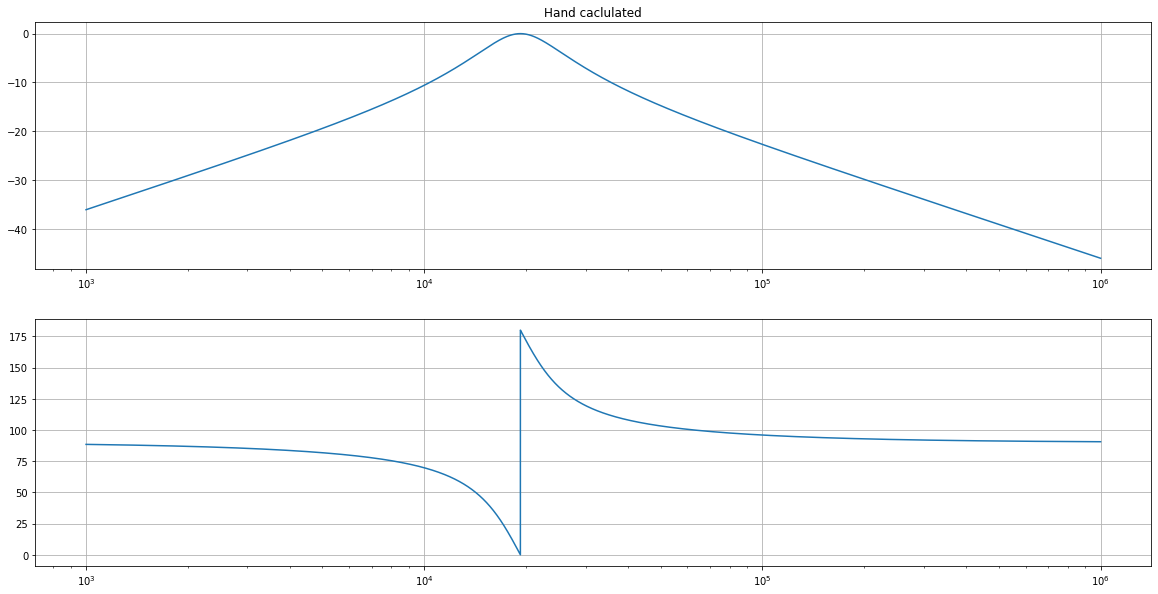
\includegraphics[width=7in]{/home/zachariahmus/Documents/Code_Projects/ECE351/ECE351/Lab10/Figure 2023-04-26 121422.png}

If we use the built in functions we produce the following graph: \vspace*{12pt}

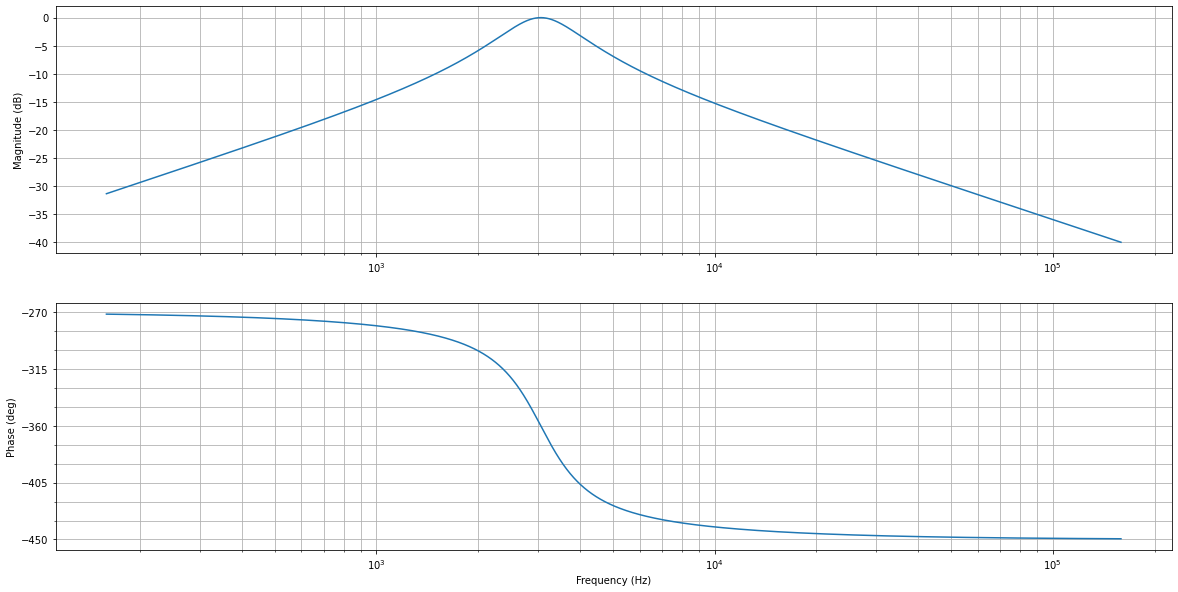
\includegraphics[width=7in]{/home/zachariahmus/Documents/Code_Projects/ECE351/ECE351/Lab10/Figure 2023-04-26 121418.png} \vspace*{12pt}

The last thing to do is to run a signal through this filer to see what happens: \vspace*{12pt}

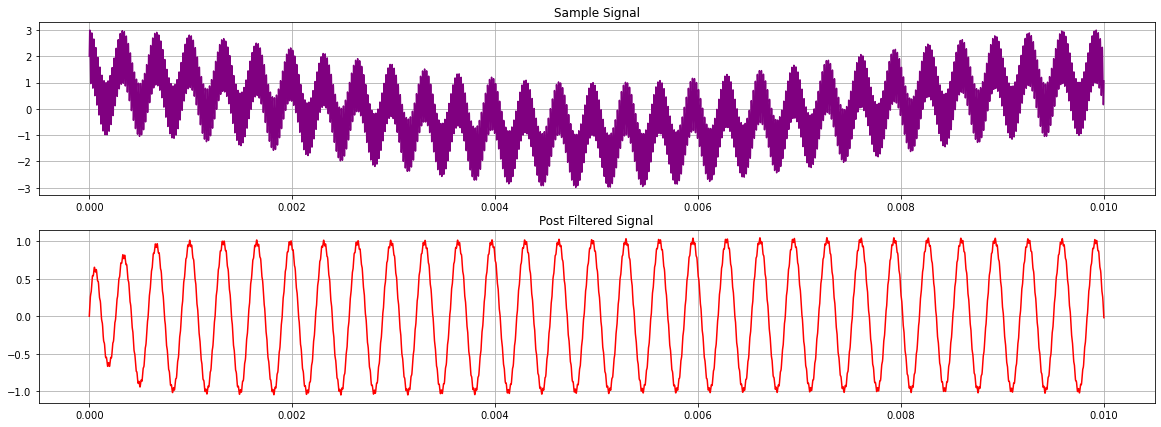
\includegraphics[width=7in]{/home/zachariahmus/Documents/Code_Projects/ECE351/ECE351/Lab10/Figure 2023-04-26 121412.png} \vspace*{12pt}

\section*{Questions}
1. Explain how the filter and filtered output in Part 2 makes sense given the Bode plots from
Part 1. Discuss how the filter modifies specific frequency bands, in Hz. \vspace*{12pt}

Given the bode plot, we have a narrow range band-pass filter. The input signal is comprised of many frequencies, and the output looks like a single frequency. This makes sense as the filter only allowed through the single frequency in the pass-band. 


2. Discuss the purpose and workings of
scipy.signal.bilinear() and scipy.signal.lfilter().\vspace*{12pt}

The bilinear function takes a transfer function and converts into the z domain, and the lfilter function is used to filter a function through the filter using the given z domain transfer function. 

3. What happens if you use a different sampling frequency in scipy.signal.bilinear() than
you used for the time-domain signal? \vspace*{12pt}

The time domain signal resolution is related to the sampling frequency, so if the frequency increased then so would the time domain function resolution, with the opposite also being true. 

\section*{Conclusion}
In this lab we were able to create a transfer function from a given circuit. Using that transfer function we were then able to transform it to the z domain and use that to filter a signal through it. This process makes filtering a signal much faster and easier than trying to convolve the transfer function with the signal as the signal is not apparently a regular signal. This allows us to check the functionality of our band pass filter easily. 



\end{document}
